\documentclass[chapter, oneside]{oblivoir}
\usepackage{kotex}
\usepackage{graphicx}
\usepackage{mathtools}
\usepackage{amsmath}
\usepackage{amssymb}
\usepackage{amsthm}
\usepackage{hyperref} 
\hypersetup{colorlinks=false,}  
\usepackage{fapapersize}
\usefapapersize{210mm, 297mm,30mm,*,35mm,30mm}

\title{자기주도학습과제}
\author{esctabcapslock}
\date{June 2021}

\begin{document}

\maketitle


\begin{abstract}
    자기주도학습과제입니다! 06.26부터 06.29까지 나흘동안 하루에 두세편씩 작성했습니다. 금방 걸릴 줄 알았는데 생각보다 오려걸렸네요. 근데 이게 자기주도학습과제의 전부가 아니라니...무섭군요. 하여튼 즐겁게 읽어주세요. 장 수는 21장이지만 \LaTeX 특성상 공백이 많아서 생각보다 분량은 많지 않아요. 수식 포함 15,000자 정도? 아프지 않게 금방 끝날겁니다. 틀린거 있으면 알려주세요.
\end{abstract}



\chapter{자기주도적 학습 과제 1 (12.1-4)}

\section{수학에서 ‘공간(space)’이란 어떤 의미를 갖나요? `공간을 정의한다’라는 것은 무슨 뜻인가요?}
\paragraph{공간}
	특별한 속성과 몇 가지 부가적 구조를 갖는 집합
\paragraph{구조}
	임의의 집합이 주어졌을 때 여기에 부여한 수학적 성질로 인해 그 집합이 갖추게 되는 형태

\section{‘유클리드 공간’의 정의는 무엇인가요?}

\paragraph{}{영문 위키의 정의}
\begin{itemize}
    \item 유클리드의 평행선의 공리와 피타고라스의 정리가 성립하는 $n$차원 공간
    \item 유클리드가 생각했던 거리와 길이와 각도를 좌표계를 도입하여, 임의 차원의 공간으로 확장한 것
\end{itemize}

\paragraph{국문 위키의 정의}
\begin{itemize}
    \item 유한 차원의, 실수 기반, 내적이 정의된 벡터 공간 $\mathbb{R}^n$ 은 $\mathbb{R}$을 $n$회 데카르트 곱한 집합이다.
    \item 그 위에서, 내적은, $\left\langle u,v \right\rangle=\sum_{i=1}^{n}{u_iv_i}$로 정의
\end{itemize}
	
\section{내적의 `기하적 정의'와 `대수적 정의'를 비교하고 동치임을 증명하시오.}

\paragraph{기하학적 방법}
\begin{itemize}
    \item 직관적임
    \item 엄밀하지 않으며, 갈이가 $0$일 때, 예외가 생겨서 정의가 아름답지 않음.
    \item N차원 확장이 불편함 (4차원 으악 ㅠㅠ)
    
\end{itemize}

\paragraph{대수적 방법}
\begin{itemize}
    \item 엄밀하게 정의할 수 있음
    \item $N$차원으로 쉽게 확장할 수 있다.
    \item 비-작관적
\end{itemize}
	
	
\paragraph{동치 증명}

두, 벡터 $a, b$를 생각하자.
$\left|a\right|\left|b\right|=0$이면, 두 정의 모두 $a \cdot b=0$ 이 되는 것은 자명하다.

아닌 경우를 생각하자.

제2코사인 정리에 의해서, 

$$|a|^2 + |b|^2 - |a-b|^2 = 2ab \cos \theta$$
$$\sum_{i=0}^{n-1} a_i^2 + \sum_{i=0}^{n-1}b_i^2 - \sum_{i=0}^{n-1} \left(a_i-b_i\right)^2$$
$$=\sum_{i=0}^{n-1}a_i^2+\sum_{i=0}^{n-1}b_i^2-\sum_{i=0}^{n-1}a_i^2-\sum_{i=0}^{n-1}b_i^2+\sum_{i=0}^{n-1}{2a_ib_i}$$
$$=\sum_{i=0}^{n-1}{2a_ib_i}= a \cdot b =2\left|a\right|\left|b\right|\cos \theta$$
따라서, 두 정의는 동치이다.

\section{외적의 `기하적 정의'와 `대수적 정의'를 비교하시오.}

\paragraph{기하적 방법}
\begin{itemize}
    \item 직관적이다.
    \item 각도가 주어진 경우 편함
    \item 각도를 모른다면 삼각함수의 지옥을 맛볼 수 있음.
\end{itemize}


\paragraph{대수적 방법}
\begin{itemize}
    \item 정의가 간편
    \item 행렬식과 연관 지을 수 있어 행렬식의 성질을 이용할 수 있음.
    \item 높은 차원으로 확장하기 쉽다.
\end{itemize}


\paragraph{동치성 증명}


	1차워 공간에서는 자명하다
	3차원 공간에서의 증명은 다음과 같다. (그 이상은 교과서에다 다루지 않는다.)
	두, 벡터 $a$, $b$ 생각.
	$\left|a\right|\left|b\right|=0$ 이면, $a \times b =0$은 자명하다.
	
	아닌 경우를 생각하자.
	$$\left|a\right|^2\left|b\right|^2-\left|a\times b\right|^2=\left(a_1^2+a_2^2+a_3^2\right)\left(b_1^2+b_2^2+b_3^2\right)-\left(|a_2b_3-a_3b_2,\;a_3b_1-a_1b_3,\;a_1b_2-a_2b_1|\right)^2$$
	$$= a_1^2b_1^2+a_2^2b_2^2+a_3^2b_3^2+\left(a_1^2b_2^2+a_2^2b_3^2+a_3^2b_1^2+a_1^2b_3^2+a_3^2b_2^2+a_2^2b_1^2\right)-$$$$  \left(a_2^2b_3^2+a_3^2b_2^2+a_3^2b_1^2+a_1^2b_3^2+a_3^2b_1^2+a_1^2b_3^2\right)+2\left(a_2b_2a_3b_3+a_3b_3a_1b_1+a_1b_1a_3b_3\right)$$
	$$=a_1^2b_1^2+a_2^2b_2^2+a_3^2b_3^2+2\left(a_2b_2a_3b_3+a_3b_3a_1b_1+a_1b_1a_3b_3\right)$$
	$$= \left(a_1b_1+a_2b_2+a_3b_3\right)^2=a\cdot b$$
	$$\therefore |a\ \times b|^2\ =\ |a|^2\ |b|^2\ -\ |a\ \cdot b\ |^2\ =\ \ |a|^2\ |b|^2\ -\ |a|^2\ |b|^2\ cos^2\ \theta$$
	$$=\ |a|^2\ |b|^2\ sin^2\ \theta$$
	$$\therefore\left|a\times b\left|=\left|a\right|\right|b\right|\left|sin\theta\right|$$

\section{이차원 벡터의 외적을 정의할 수 있는가}

\paragraph{기하적 관점에서 고찰}


외적의 결과는 두 벡터의 수직이여야 함.

그 결과가 같은 평면 위에 있다면, 각도의 덧셈 상에서 모순이 발생함.

따라서 모순임.

    

\chapter{자기주도적 학습 과제 2 (12.5-6)}

\section{$\mathbb{R}^3$에서 거리 구하는 공식 만들고 $n$차원 확장}

$p _{0} + q _{0} t$과  $p _{1} + q _{1} t$ 생각하자

\paragraph{3차원에서의 거리공식}
두 직선이 만드는 평면의 법선벡터를 생각한다. 직선 위 임의의 두 점을 잇는 벡터를, 
이 법선벡터에 사영시킨 것이 바로 거리가 될 것이다.

$\left| \mathrm{proj} _{q _1 \times  q _{2}} ( p _{1} - p _{2} ) \right|$

\paragraph{$n$차원 확장 방법 1}

해가 존재한다면, $q_0$, $q_1$은 평행하지 않다.
$q_0$, $q_1$, $p_0 - p_1$을 세 기저로 하는 공간을 생각할 수 있고,
만일 그렇다면, 나머지 기저들은 거리 공식에 영향을 다 못 줄 것(싹 다 0임). 
이 기저들을, 가우스-조르단 방법 하듯이 하듯 잘 손질하면 
수직인 세 백터로 만들 수 있을 것이고, 그러면 3차원 백터가 나오니까 위의 공식에 대입한다!

\paragraph{$n$차원 확장 방법 2}
2학년 1학기 일반물리학 실험때 배운 최소제곱법 유도방식을 이용하자.

저 두 직선을 빼면, $a+bs+ct$꼴이며, 거리의 제곱을 구하면, $\sum \left( a(n) + b(n)s + c(n) t \right)^2 $이며,
$s$와 $t$에 각각 편미분 해주면, 2원 1차 연립방정식의 꼴이 된다. 따라서, 
$\begin{bmatrix} s \\t \end{bmatrix}$ $ =- \begin{bmatrix} \Sigma  ab \\ \Sigma  ac  \end{bmatrix} \begin{bmatrix} \Sigma  b ^{2}& \Sigma  bc \\ \Sigma  bc& \Sigma  c ^{2} \end{bmatrix}  ^{-1} $로 어떤 값을 구할 수 있으며, 거리는 와 가 무한하면 무한하며, 대충 아래로 볼록한 이차식 형태꼴로 나오는 것으로 예상되며, 저 값이 최소값이라고 추측된다.
따라서, 저 $s$와 $t$를 대입한 거리값이 최소값일 가능성이 매우 높다.


\section{곡선의 정의}

\paragraph{위키피디아 정의}  

연속적인 점들의 집합이다.

구간 $I$와 위상공간 $X$가 있을 때, $I \to X$의 연속함수
\paragraph{위상공간} 
어떤 점의 근처(근방)가 무엇인지에 대한 정보를 담고 있지만, 점 사이의 거리나 넓이·부피 따위의 정보를 포함하지 않는 공간.

\paragraph{근방}
어떤 점의 주위를 포함하는 집합. 위상공간 $X$속 점 $x \in X$의 근방은 $x$를 원소로 포함하는 열린 부분집합이다.

\paragraph{선생님 PPT}
사상 $\left[ a, b\right] \Rightarrow \mathbb{R}^n$에 대해, $t$가 $\left[ a, b\right]$에서 변할 때, 점들의 모임
\section{페아노 곡선의 정의와 성질}

\begin{figure}[h!]
    \centering
    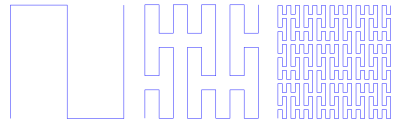
\includegraphics[width=.7\textwidth]{img/peano.png  }
    \caption{페아노 곡선의 모습}
    \label{texlive:exdit}
\end{figure}

자연수를 정의하여 수많은 수학덕을 양성(?)한 것으로 유명한 이탈리아 수학자 주세페 페아노가 1980에 발견한 곡선이다. 
단위 길이를 단위 평면에 대응시키는 전사 함수이다. 
칸토어가 $\mathrm{Card}(N)=\mathrm{Card}(N ^{2})$ 증명하는데 영감을 줬다고 한다.
공간충전곡선(空間充塡曲線)의 한 예이며, 교점 없이 평면공간, 더 나아가 임의의 폐집합 내를 체우는 곡선이다. 


\section{타원면과 만나는 평면의 방향과는 상관 없이 교차하는 부분은 타원인가}

중명 1.
$x ^{2} /a ^{2} +y ^{2} /b ^{2} +z ^{2} /c ^{2} =1$과, $a' x+b' y+c' z=d$ 두 선의 교점이라고 생각하자. 평면의 식을 $z$에 대해 정리한 뒤, 첫 번째 공식에 대입하게 되면, $x^2$, $y^2$, $x$, $y$등이 담긴 방정식이 나온다. 근데, 
\begin{enumerate}
    \item  $x^2$과 $y^2$의 부호가 같을 것이 자명하다. 
    \item 타원의 경우 정의역이 제한되어 있기 때문에, 결과 식도 어느 범위로 재한되어 있으며, 이를 만족하는 이차함수는 타원이 유일하니까
\end{enumerate}
$\to$ 결과는 타원이다.

이는 교선을 $xy$평면에 사영시킨 것인데, 원래 교선도 어떤 평면 위에 있으니까,
$xy$평면에서 거리에 관한 공식들이, 어떤 평면과 $xy$평면의 이면각 $\theta$에 대해, $\cos(\theta)$에 비례하는 형태를 띄게 된다. 
따라서, 두 초점 사이 거리 관계가 $xy$평면에서 성립하면, 원래 평면에서도 성립하므로, 원래 평면에서 그려진 교선은 타원이다.

\section{카발리에리의 원리로 타원면으로 둘러싸인 부분의 부피 구하는 공식을 만들기. 그리고 $n$차원으로 확장하시오.}
타원 면적 구하는 공식은 $\pi a b$이다.

타원면을  $ \frac{x ^2}{a^2} +\frac{y^2}{b^2} + \frac{z^2}{c^2} =1$로 잡자.

$z=z$인 평면을 기준으로 생각하면, $1 - \frac{z ^{2}}{c^2} = \frac{x ^2}{a^2} +\frac{y^2}{b^2}  $이니, 면적은 $\pi ab \sqrt {1-z ^{2}}$이다.

이는 $\pi \sqrt {1-z ^{2}}$를 $ab$배 한 것이니, 
구하구자 하는 부피는 카빌리에리 원리에 의해 $1- \frac{z^2}{c^2} =x ^{2} +y ^{2}$ 의 부피의 $ab$배 일 것이다.
이걸 $-c$부터 $+c$까지 적분하면 $\frac{4}{3}\pi c$이며, 따라서 타원면의 면적은 $\frac{4}{3}\pi abc$이다.
\chapter{자기주도적 학습 과제 3 (13.1, 14.2)}
참고. 이 장에서 따른 말이 없으면, $V$는 $n$차원 유클리드 공간을 의미하며, $D$는 $V$의 부분집합이다.
$f$는 $f: D \to V$인 함수이다. 그리고$p \in D$, $L \in V$라고 하자.
그리고 $\left\{ x_k \right\}$는 수열이다.

\section{$V$의 두 점 $p$, $q$ 사이의 거리 구하는 공식}

$p = \left\langle p_1, p_2 \cdots p_n \right\rangle$, $q = \left\langle q_1, q_2 \cdots p_n \right\rangle$라 둘 때,

$$\mathrm{d}(p,q) =  |p-q| = \sqrt{\left(p_1^2 - q_1^2\right)^2 + \left(p_2^2 - q_2^2\right)^2 + \cdots + \left(p_n^2 - q_n^2\right)^2 }$$으로 구할 수 있다.


\section{``$x \to p \Rightarrow f(x) \to L$이다''의 엄밀한 정의}  \label{chap:imt}
$\epsilon$-$\delta$ 논법 비슷하게 정의하면 될 것 같다.

$\forall \epsilon > 0$, $\exists \delta > 0$, s.t. $|p-x|< \epsilon \Rightarrow |L - f(x)| < \epsilon$

\section{``$f$가 $p$에서 연속이다''의 엄밀한 정의}
$x \in D$, $x \to P$이면, $f(x) \to f(P)$일 때 연속이라고 정의하자.

\section{$x_k \in V$이다. 이때 “$k \to \infty \Rightarrow x_k \to L$이다”의 엄밀한 정의}  \label{chap:inf}

$\forall \epsilon > 0$, $\exists M > 0$, s.t. $k > M \Rightarrow |f(x_k)-L| < \epsilon$

\section{ $x_k \in D$이다. ``$( k \to \infty \Rightarrow x_k \to p ) \land ( x \to p \Rightarrow f(x) \to L)$ $\Rightarrow$ $(k \to \infty \Rightarrow f(x_k) \to L)$''를 증명}

$\forall \epsilon > 0$,  자연수 $M$을 다음과 같은 방식으로 잡자.

그리고, \ref{chap:imt}\sectionname 에서 보인 바와 같이 $|p-x_k|< \epsilon \Rightarrow |L - f(x_k)|$를 만족하는 양수 $\delta$를 잡을 수 있다.
\ref{chap:inf}\sectionname 에서 보인 바와 같이 $k > M \Rightarrow |f(x_k)-L| < \delta$를 만족하는 양수 $M$를 잡을 수 있다.

이렇게 $M$을 잡게 되면, $|p-x_k|< \epsilon \Rightarrow |L - f(x_k)|$가 성립하게 되니, 
주어진 명제가 성립힌다.

\chapter{자기주도적 학습 과제 4 (6.3, 11.2, 13.1-3)}

\section{$3$차원 공간 안에 놓인 평면 $\gamma$ 위에 점 $C$를 중심으로 하고 반지름이 $r$인 원을 벡터로 나타내시오}
법선 벡터를 $n$이고 했을 때, 이 벡터에 수직이면서, 길이가 $r$이고 $C$를 지나면 된다.
그대로 식으로 옮기면 $\left\{ x \; | \; n \times (c - x) = 0\right\}$이 될 것이다.

\section{길이가 양수인 닫힌 구간 $I$에서 정의된 $f:I \to \mathbb{R}^3$, $\; r(t) = f(t)i+g(i)j+h(t) k$가 있다. $L=(L_1, L_2, L_3)$일 때, $\lim_{t \to p}r(t)=L$ $\iff$ $\lim_{t \to p}f(t)=L_1$ $\land$ $\lim_{t \to p}g(t)=L_2$ $\land$ $ \lim_{t \to p}h(t)=L_3 $임을 보여라}

\paragraph{$\Rightarrow$ 증명}
가정에 의해서, $\forall \epsilon >0$, $\exists \delta > 0$, $|t-p|<\delta \Rightarrow |r(t)-L|<\epsilon$이 성립함.

즉, $$\sqrt{\left(f(t)-L_1 \right)^2 + \left(f(t)-L_2 \right)^2 + \left(f(t)-L_3 \right)^2 } < \epsilon$$이 성립한다는 말이다.
그러므로, 제곱근 안에 각각의 제곱항들은 $\epsilon^2$보다 작을 것이다.

따라서, $\left|f(t)-L_1 \right| < \epsilon$,  $\left|f(t)-L_2 \right| < \epsilon$,  $\left|f(t)-L_3 \right| < \epsilon$이 성립한다.

\paragraph{$\Leftarrow$ 증명}

가정에 의해서, $\forall \frac{\epsilon}{2} >0$, $\exists \delta > 0$, $\left|f(t)-L_1 \right| < \frac{\epsilon}{2}$,  $\left|f(t)-L_2 \right| < \frac{\epsilon}{2}$,  $\left|f(t)-L_3 \right| < \frac{\epsilon}{2}$이 성립함.

즉, $$ |r(t)-L| = \sqrt{\left(f(t)-L_1 \right)^2 + \left(f(t)-L_2 \right)^2 + \left(f(t)-L_3 \right)^2 } < \sqrt{3\left(\frac{\epsilon}{2}\right)^2} < \epsilon$$이 성립한다는 말이다.

따라서 증명이 끝났다.

\section{매끄러운 곡선, 조각마다 매끄러운 곡선 뜻}
\paragraph{토머스 6.3의 정의} $f(x)$가 주어진 구간에서 연속이고 미분 가능하면 매끄러운 것임.

\paragraph{매끄러운 곡선, 토머스 13.1의 정의} 곡선 $r(t)$에 대해, 정의역의 모든 점에서 $r(t)$와 $\frac{dr}{dt}$가 연속이고, $\frac{dr}{dt}>0$
\paragraph{조각마다 매끄러운 곡선, 토머스 13.1의 정의} 매끄러운 곡선을 연결한 것.

\section{곡선의 길이 정의. 정의역의 길이가 무한대인 열린 구간인 매끄러운 곡선의 길이가 유한일 수 있을까}
\paragraph{곡선의 길이, 토마스} 매끄러운 곡선 $r(t) = x(t)i+y(t)j + z(i)k$에서, 곡선의 길이 $L$은  
$$\int_a^b \sqrt{ \left( \frac{dx}{dt} \right)^2 + \left( \frac{dy}{dt} \right)^2 + \left( \frac{dz}{dt} \right)^2 }$$
로 정의된다.

그리고, 조각마다 매끄러운 곡선의 경우, 조각들의 길이의 합으로 정의하면 될 것 같다.

\paragraph{길이를 갖는 곡선(rectifiable curve)}
해석학적으로는, 길이를 다른 방법으로 정의할 수 있다. 
구간 $I = \left[a,b\right]$를 분할한 것을 $P = \left\{ a=x_0, x_1 \cdots x_n=b \right\}$이라고 하자. $r : I \
to \mathbb{R}^n$이 때,
$||p|| \to 0$일 때, $$\sum_{k=0}^{n-1} d(x_k, x_{k+1})$$의 상한을 길이로 정의할 수 있다. 

(삼각부등식에 의해서, 노름이 0에 수렴할 경우, 주어진 식은 커지게 된다.)

\paragraph{정의역이 무한대인 유한직선}
만약 무한한 분할을 잡을 수 있다고 한다면,
$I = [0, \infty] $이고, $r(t) = \left\langle \tan^{-1}(x) \right\rangle$로 잡으면,
$$\lim_{n \to \infty} \sum_{k=0}^{infty} tan^{-1}(\frac{k+1}{n}) - tan^{-1}(\frac{k}{n}) = \lim_{m \to \infty} tan^{-1}(m) - tan^{-1}(0) = \frac{\pi}{2} $$
이니까 유한하지 않을까?

$\mathrm{Card}([0,1]) = \mathrm{Card}([0,\infty])$가 아닌가.

\section{13.3 - 13.4 학습지 13번 문제 참조}

$1 over {n \pi}$꼴로 분할을 잡은 뒤, 극대, 극소값들을 잘 연결해서 위로 유계임을 보이면 된다. 수업시간에 했으니 생략.

(참고로 답은 $p>1$이다.)


\chapter{자기주도적 학습 과제 5 (13.4-5, 14.1-3)}
\section{곡선의 곡률(curvature)과 비틈림률(torsion)의 정의}

\paragraph{곡률}
곡선 $r(t)$에 대해, 단위접벡터 $T$는 $\frac{dr / dt }{ \left| dr / dt\right|}$로 정의한다.
이는, 곡선에 접하는 원(접촉원)의 반지름의 역수와 같다.

그리고 이 곡선의 곡선길이 매개변수를 $s$라고 할 때, 곡률 $\kappa$는 $\left| \frac{dT}{ds}\right|$로 정의한다.

\paragraph{비틀림률}
주 단위 접선 벡터를 $N = \frac{1}{\kappa}\frac{dT}{ds}$로 정의하고, 종 법선벡터를 $B = T \times N$로 정의한다. 이때, 비틀림률 $\tau$는 $\tau = -\frac{dB}{ds} \cdot N $로 정의한다.
이는, $T$와 $B$가 이루는 평면에서 얼마나 곡선이 벌어지는지를 나타난다. (공간적으로 얼마나 휘어 있는지를 나타낸다.)

\section{열린 집합, 닫힌 집합, 연결 집합의 정의, 집합의 연산 관련 성질 }
\paragraph{내부점 (쌤 ppt)}
$G \subset \mathbb{R}^n$과, $p \in G$에 대해서, $\exists \delta > 0 $ s.t. $\left\{ x \in \mathbb{R}^n \; | \; \left|x-p\right|<\delta \right\} \subset G$면, $p$를 $G$의 내부점이라 한다.



\paragraph{경계점 (쌤 ppt)}
$\forall \delta > 0 $ s.t. $\left\{ x \in \mathbb{R}^n \; | \; \left|x-p\right|<\delta \right\} \cap G \ne \varnothing$고, $\left\{ x \in \mathbb{R}^n \; | \; \left|x-p\right|<\delta \right\} \cap G^c \ne \varnothing$면, $p$를 $G$의 경계점이라 한다.

\paragraph{열린집합 (쌤 ppt)}
자신의 모든 점들이 내부점인 집합

\paragraph{닫힌집합 (쌤 ppt)}
자신의 경계점들을 모두 원소로 갖고 있는 집합

\paragraph{성질 (쌤 ppt)}
열린집합, 혹은 닫힌집합끼리는 유한번의 합집합, 교집합 연산에 대해 닫혀있다.
그러나, 열린집합은 무한 합집합만 열린집합이며, 닫힌집합은 무한 교집합만 닫힌집합니다.

\paragraph{연결 공간 ( 한국어 위키피디아)}
공집합이 아닌 두 열린집합으로 쪼갤 수 없는 집합이다.

또, $x,y \in X$인 집합 $X$내 연속함수 $f: [0,1] \to X$가 존재해 $f(0)=x$, $f(1)=y$를 만족하면 거리연결공간이라고 한다.
유클리드 공간의 경우, 연결 공간과 거리연결공간은 필요충분조건임이 증명되어있다.

\paragraph{연결 공간의 연산}
연결공간의 합집합은 연결공간이 되지 않을 수 있다. $\left\{ (x,y) |  x^2 + y^2 < 1 \right\}$과  $\left\{ (x,y) |  (x-3)^2 + y^2 < 1 \right\}$ 각각은 연결 공간인데, 합집합은 연결 공간이 아니다. (쪼개는 것이 가능하다.)

연결공간의 교집합도 연결공간이 되지 않을 수 있다. 두 집합의 교집합이 서로 떨어져 있을 수 있기 때문이다.

\section{$U \subset \mathbb{R}^2$은 는 공집합이 아닌 열린 연결 집합이다. $f: U \to \mathbb{R}$일 때, 점 $p \in U$에서 $f$의 편미분의 정의}
\paragraph{$x$에 관한 편미분}
$$\left.\frac{\partial f }{\partial x} \right|_{p} = \lim_{h \to 0} \frac{f(p+hi)-f(p)}{h}$$로 정의한다. 이는, $x$축에 평행하게 함수를 잘랐을 대, 이 함수의 기울기라고 할 수 있다.
$y$에 대해서도 대징적으로 성립한다.
\section{편미분가능하면 연속인가. 어떤 조건이 더 필요한가}

\paragraph{반례}
당연히 편미분 가능하면 연속이 아니다. $f(x,y)$를 다음과 같이 정의하면, 원점에서 연속이 아닌 것이 자명하다.
$$f(x) = \begin{cases}
    1, & xy=0 \\
    0, & xy \ne 0
\end{cases}
$$로 정의하면 된다.

\paragraph{추가조건}
심지어 방향미분계수가 존재해도 연속이 아니다. 음...

\section{이변수 함수의 미분계수는 몇차원인가}
실수라면, 2개의 값으로 표현해야 할 것 같다. 어느 방향으로 기울어졌는지에 관한 정보가 필요하기 때문이다. 
\chapter{자기주도적 학습 과제 6 (14.4-5)}
\section{함수가 가진 변수의 개수에 상관 없이 하나의 식으로 연쇄법칙을 나타낼 수 있을까요}
실은 하나의 식이라고 생각한다. 그냥 모든 변수에 대해 미분한 어떤 식이 있을 수 있고,

적당히, 독립인 변수들은 서로의 미분이 0임을 넣어 주면 될 것 같다.

\section{방향도함수의 정의와 기하학적 의미}
점 $p=(x_0, y_0)$에서 $u$ 방향의 방향미분계수는 다음과 같이 정의된다.

$$(D_u f)_p = \lim_{h \to 0} \frac{f(p+hu) - f(p)}{h}$$
이 값을 갖는 함수를 방향도함수로 정의한다.

이 값은, 어떤 함수를 $p$와 평행하게 자른 단면에서의 기울기를 나타내는 것이다.

\section{기울기 연산의 정의과 기하학적 의미}
점 $p=(x_0, y_0)$에서 $f$를 기울기 연산한 것은 다음과 같이 정의한다.
$$\nabla f  = \frac{\partial f}{\partial x}i + \frac{\partial f}{\partial y}j$$

이는, $f$가 증가하는 방향을 나타낸다.
\section{$f: \mathbb{R}^2 \to \mathbb{R}$이고, 0에서 모든 방향의 방향미분계수 갖으며, 0에서만 불연속 함수찾기}
$f(0,0)=0$으로 정의하자. 0에서 연속 아니지만 미분방향계수 존재하는 '그' 문제 생각. 그 문제에서 불연속적인 부분을 깍아서 매끄럽게(?) 만들면 되지 않을까 생각.
$$f(x,y) = \begin{cases}
    e^{\left|\frac{x-y^2}{y^3} \right|} & y \ne 0\\
    0, & y = 0
\end{cases}
$$


\begin{figure}[h!]
    \centering
    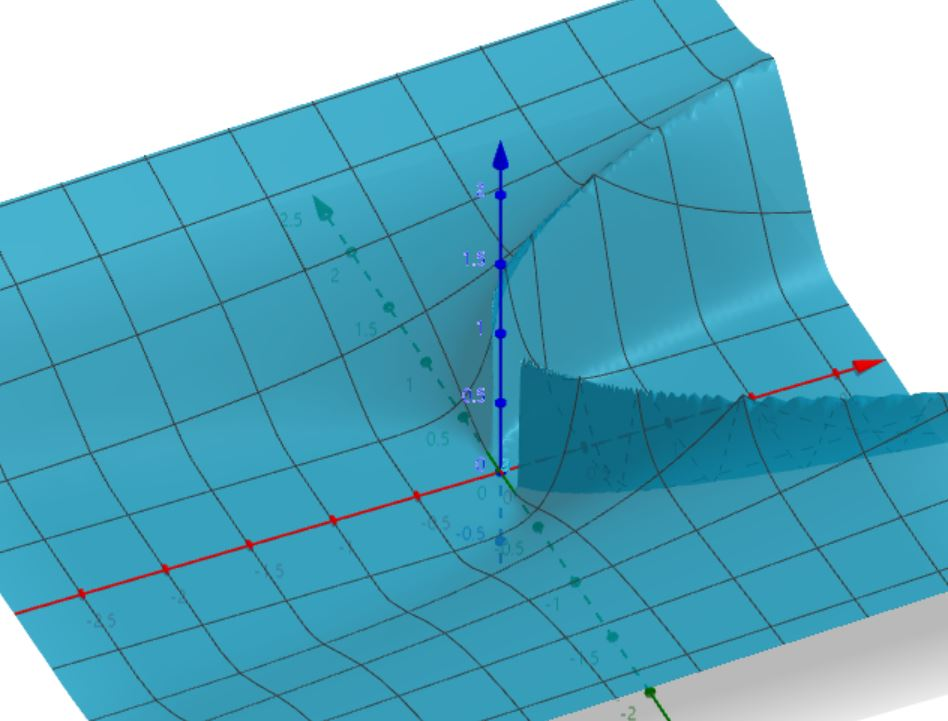
\includegraphics[width=.7\textwidth]{img/strange.JPG  }
    \caption{대충 이렇게 생김}
    \label{texlive:exdit}
\end{figure}
\paragraph{증명}
$u=(0,1)$에 대하여,
$$lim_{h \to 0} \frac{f(0,0)-f(h,kh)}{h} = lim_{h \to 0} \frac{e^{-1/|h|}}{h} = 0$$

$u=(1,k)$에 대하여는, '그'문제 증명하듯이 증명하면 됨.

하지만, $x=y^2$라면, $f(x,y)=1$이므로, 안됨,


\section{복소함수의 미분과 편미분}
미분은 똑같이 정의한다.
$$f'(z) = \lim_{\Delta z \to 0} \frac{f(z_0 + \Delta z) -f(z_0)}{\Delta z}$$
실수축과 허수축에 대해 편미분(?) 할 수 있는 것 같다.

\chapter{자기주도적 학습 과제 7 (13.3~6)}

\section{단위속력곡선 뜻, 속력이 0이 되지 않는 매끄러운 곡선은 단위속력곡선이 되도록 재매개화 가능 증명}
\paragraph{단위속력곡선}
$\frac{dr}{ds} = 1$이 되게끔 $s$로 재매개화 한 곡선이다. 

\paragraph{증명}
조건에 의해, $\left| \frac{dr}{dt} \right| > 0$이며, 이 값은 연속적이다. 따라서, 적분할 수 있다.
$s = \int_0^{t_0} \left| \frac{dr}{dt} \right|  dt$로 정의할 수 있다. 
이 함수는 증가함수이기 때문에, 당연히 역함수가 존재한다. 따라서 $t = f(s)$라고 둘 수 있다.

따라서, $r(f(s)))$로 곡선을 재매개화 하게 되면, $s$로 미분했을 때, $ \left| \frac{d (r(f(s)))}{ds} \right| = \left|\frac{dr}{dt}\left| \frac{dt}{dr}\right| \right| = 1$이 되게 된다. 증명 끝.


\section{$T$, $N$, $B$를 4차원 공간에 놓인 곡선으로 확장}
이 이하는 , `Raffles Junior College'의 `Lee Mun Yew '가 작성한 `Curves in Four-Dimensional Space'을 참고한 것임을 밝힌다.


일단, $T$와 $N$은 큰 무리 없이 정의할 수 있는 것처럼 보인다. 그런데 이 둘에 수직한 벡터는 어떻게 구할까. 외적을 사용하긴 어렵다. 수직한 공간의 기저가 2개이기 때문이다.

$$B = \frac{dN}{dS} - \left(\frac{dN}{ds} \cdot T\right)T -  \left(\frac{dN}{ds} \cdot N\right)N$$으로 $B$를 정의한다. 
이것은 마치, 선형 대수 시간에 배운 그람-슈미츠 직교화 과정을 보는 것 같은 느낌이다. (두 벡터의 수직인 어떤 벡터를 잡는 그런 느낌이다.)

하지만 4차원은 기저가 4개이므로, 하나를 더 잡을 수 있는데, 그것을 $D$라고 잡았다.

\section{$\tau$와 $\kappa$를 4차원 공간에 놓인 곡선으로 확장}
$\tau$와 $\kappa$는 위 정의대로 하면, 3차원의 것을 그대로 정의할 수 있을 것으로 보인다. 그리고, 하나가 더 필요하다.
이 보고서에서는 $\sigma$라는 값을 하나 더 도입해서 해결한다.
$$\sigma D = \frac{dB}{ds} - \left(T \cdot \frac{dB}{ds}\right)T - \left(N \cdot \frac{dB}{ds}\right)N - \left(T \cdot \frac{dB}{ds}\right)B $$


\section{$\tau = 0$이면, 그 곡선은 한 평면 위에 놓여 있음 증명}
정의에 의해서, $\frac{dB}{ds} = \tau N = 0$이므로, $B$는 일정하다! 따라서, $T$와 $N$이 이루는 평면은 일정하다. 근데$r$은 $T$와 $N$위에서 움직이므로, (속력이 이 두 벡터에 대해 표현할 수 있기에,,,)결국 한 직선 위에 움직인다.
\section{3차원 공간에 구면좌표계가 주어졌을 때, 이 공간에 놓인 매끄러운 곡선의 속도와 가속도 구하는 공식 }
위키피디아에 따르면,

$$\hat{r} = \cos \theta \sin \phi \hat{x} + \sin \theta \sin \phi \hat{y} + \cos \phi \hat{z}$$
$$\hat{\theta} = - \sin \theta \hat{x} + \cos \theta \hat{y} $$
$$\hat{\phi} = \cos \theta \cos \phi \hat{x} + \sin \theta \cos \phi \hat{y} - \sin \phi \hat{z}$$
에 있을 때,

$$\mathbf{r} = r \hat{\mathbf{r}}$$

$$\mathbf{v} = \dot{r} \hat{\mathbf{r}} + r \dot{\theta} \sin \theta \hat{\mathbf{\theta}} + r \dot{\phi} \hat{\mathbf{\phi}} $$

$$\mathbf{a} = \left(\ddot{r} - r \dot{\phi}^2 - r \dot{\theta}^2 \sin^2 \phi \right)\hat{\mathbf{r}} + \left(r \ddot{\phi} + 2 \dot{r} \dot{\phi} - r \dot{\theta}^2 \sin \phi \cos \phi \right) \hat{\mathbf{\theta}} + \left( r \ddot{\theta} \sin \phi + 2 dot{r}\dot{\theta} \sin \phi + 2 r \dot{\phi}\dot{\theta} \cos \phi \right) \hat{\mathbf{\phi}}$$
가 된다. 무섭게 생겼다.
\chapter{자기주도적 학습 과제 8 (14.5-7)}
\section{국소극값과, 절대극값}
\paragraph{극소극값}
점 $a,b$를 중심으로 하는 원 $S$가 존재해허, $(z,y) \in S$에서,  $f(a,b) \le f(x,y)$를 만족하면, 극솟값, 반대면 극댓값이라고 한다.

\paragraph{절대극값}
정의역 $D$의 모든 점 $(x,y)$에서,  $f(a,b) \le f(x,y)$를 만족하면, 최솟값, 반대면 최댓값이라고 한다.
\section{$\varnothing \ne D \subset \mathbb{R}^2 $에서, $f: D \to \mathbb{R}$이다. `$f$는 $D$의 모든 점에서 국소극댓값과 국소극솟값을 가진다.' 가능하냐.}
$f(x,y)=0$이이면, 어떤 정의역의 부분집합$S$와 원소 $(x,y) \in S$에 대해서, $f(a,b) \le f(x,y)$이지, $f(a,b) \ge f(x,y)$이니, 모든 점에서 극댓값과 극솟값을 갖는다.

\section{$f: \mathbb{Q} \to \mathbb{R}$, $f: x \mapsto cos (x)$는 어디서 극값을 갖는가}
$(0,1)$에서만 극값을 갖는다. 실수를 정의역으로 갖는 일반적인 코사인함수는 $x=n \pi$꼴에서 극값을 갖는다. 하지만, $n!=0$인 경우, $n \in \mathbb{Q}$일 때, $n \pi$는 무리수이다.
따라서, 이 수에 가장 가까운 유리 $x$를 잡는다고 해도, 실수의 완비성에 의해, 이 실수보다 $n \pi$더 가까운 유리수를 잡을 수 있다. 그리고, 이 값은 $f(x)$보다 더 $f(n\pi)$에 가까울 것이다. 따라서, 이 경우에는 극값을 잡을 수 없다.

\section{이변수 함수의 일차근사함수}
$f(a+h, b+k) = f(a,b) +  \left| \left(hf_x + kf_y\right)\right|_{(a,b)}$

\section{이변수 함수의 이차근사함수}
$f(a+h, b+k) = f(a,b) +  \left.\left(hf_x + kf_y\right)\right|_{(a,b)} +   \left.{{1} \over {2!}} \left(h^2 f_{xx} + 2hk f_{xy}+ k^2 f{yy}\right) \right|_{(a,b)}$
\chapter{자기주도적 학습 과제 9 (2.5, 10.2, 14.1)}
$D$는 $\mathbb{R}^2$의 부분집합을 나타냅니다.
\section{닫힌집합 $D$ 내부에 수렴하는 수열의 수렴값은 집합 내부에 있다. (힌트: 여집합의 내부점, 모순)} \label{chap:sub}

$L \not\in D$면  $L \in \mathbb{R}^2 \setminus D$이다. 정의에 의해 $L$은 $\mathbb{R}^2 \setminus D$의 내부점, 아니면 경계점이 된다. 경계점일 경우, $D$의 경계점도 되므로 모순이다. 따라서 $L$은 $\mathbb{R}^2 \setminus D$의 내부점이다. 따라서 적당한 양수 $\epsilon$이 존재해서, $|L-x|<\epsilon$인 점들은 역시 $\mathbb{R}^2 \setminus D$의 내부점이다. 그렇다면
극한의 정의에 의해, $\forall \epsilon >0$에서, $\exists M > 0$이여서 , $x_k \in D, k>M \Rightarrow  \left|L - f(X_k)\right|<\epsilon$이다. 근데, 위의 정의에 의해 $x_k \in \mathbb{R}^2 \setminus D$이다. 모순이다.
따라서, $L \in D$이다.

\section{유계인 집합 $D$ 내부의 모든 수열은, 수렴하는 부분수열을 갖는다. (힌트: Bolzano-Weierstrass 정리)}
Bolzano-Weierstrass 정리에 의해 성립한다. $D$를 포함하는 큰 직사각형을 잡고, 적당히 합동인 직사각형으로 쪼개는 것을 반복하며, 각 직사각형 중에는 무한한 점을 갖은 사각형이 있다.

\section{유계인 닫힌집합 $D$에서 정의된 실수값 함수도 유계이다. }
$\left\{x_k \right\}$가 유계가 아니라고 가정하자. 일관성을 잃지 않고, 그렇다면 한 점 $p$가 존재해서, $n \to \infty$일 때, $x_n \to p$이고, $f(x_n) \to \infty$이다.
근데, \ref{chap:sub}\sectionname에서 이미 $p \in D$이므로, $f(p)$가 존재해야 한다. 

$f$가 연속함수라면, 모순이다.

$f$가 연속함수가 아니라면, 다른 값을 갖는 것이 가능하다, 
\section{$f(x,y)=\sin x + \cos y$가 $\mathbb{R}^2$에서 균등연속임을 보이시오. (힌트: 균등연속 정의 줌)}
\paragraph{균등연속 정의}
$f: D \to \mathbb{R}^m$에 대해,

$\forall \epsilon > 0$, $\exists \delta >0$, $\forall s \in D$, $\forall t \in D$:

$\left(|s-t|< \delta \to |f(s)-f(t)| < \epsilon\right)$여야 한다.


\paragraph{보조정리}

$\forall x, y \in \mathbb{R}$에 대해서, 
$|x-y|<|\sin(x)-\sin(y)|$, $|s-t|<|\cos(x)-\cos(y)|$이다.
증명: MVT를 이용한다. $\sin$함수와 $\cos$함수를 미분해도 그들이니, 미분한 값의 크기는 1보다 무조건 같거나 작다.


\paragraph{증명}

$\epsilon > 0$, 
$s=(s_1, s_2),t=(t_1, t_2) \in R^2$에 대해, $|s-t|<\frac{\epsilon}{2}$면 $|s_1 - t_1|<\frac{\epsilon}{2}$이고, $|s_2 - t_2|<\frac{\epsilon}{2}$이다. 따라서,

$$|f(s)-f(t)| = \sqrt{\left(\sin s_1-\sin t_1\right)^2 + \left(\cos s_2-\cos t_2\right)} \le \frac{\epsilon}{\sqrt{2}} < \epsilon$$
이다. 따라서 균등연속이다.
\chapter{자기주도적 학습 과제 10}
$I=[a,b]$는 길이가 양수인 닫힌구간, $f$는 $I$에서 정의된 실수값 함수입니다. 다음의 (간략하게 적혀있는) 명제를 증명해야 한다.

\section{$I$는 닫힌 집합이다}
$I=[a,b]$라고 하자.($a<b$) 따라서 모든 $x \in I$는 $a \le x \le b$를 만족한다.
\paragraph{$x=a$면} 아무리 작은 $b-a>\delta>0$를 잡아도, $x-\delta \not\in I$이고, $x+\delta \in I$이다. 따라서, $x$는 경계점이다.
\paragraph{$a<x<b$면} $\delta = \min (x-a, b-a)$면, $\left\{x' | \left|x-x'\right|<\delta\right\} \in I$므로, $x$는 내부점이다.
\paragraph{$x=b$}면, $x=a$와 같은 상황이므로 x는 경계점이다.
\paragraph{그 이외의 경우}, $\delta = \min (|x-a|, |b-a|)$면, $\left\{x' \;|\; \left|x-x'\right|<\delta\right\} \in I^c$이며, $\forall \delta$에 대해서도, $x \not\in I$므로, 이는 $I$의 경계점도, 내부점도 될 수 없다.

따라서, 모든 경계점이 $I$에 포함되므로, $I$는 닫힌집합이다.


\section{항상 상합보다 하합이 크다. (분할, 상합, 하합의 정의 주어짐)}
\paragraph{분할}
$P$가 $I$의 분할이라고 하자. $P=\left\{x_0, x_1, \cdots x_n \right\}$이다. 이렇다면, $a=x_0 <x_1 < \cdots < x_n = b$가 성립한다는 말이다.


그리고,
$M_i = \mathrm{sup} \left\{ f(c_i) \;|\; x_{i-1} \le c_i \le x_i \right\}$
$m_i = \mathrm{inf} \left\{ f(c_i) \;|\; x_{i-1} \le c_i \le x_i \right\}$로 정의하자. 상한과 하한이라는 뜻이다.

\paragraph{상합} $$U(f,p) = \sum_{i=1}^n M_i \Delta x_i$$
\paragraph{하합} $$L(f,p) = \sum_{i=1}^n m_i \Delta x_i$$

\paragraph{증명}
$m_i < M_i$이다. 따라서, $m_i  \Delta x_i <  M_i \Delta x_i$이고, $\sum_{i=1}^n m_i \Delta x_i < \sum_{i=1}^n M_i \Delta x_i$이다.

따라서, $L(f,p) < U(f,p)$이다.


\section{세련분할은 원래 분할보다 상합은 작아지고 하합은 커진다.} \label{chap:hahapre}

\paragraph{보조정리} $a<b<c$일 때, $\mathrm{sup}([a,b])(b-a) + \mathrm{sup}([b,c])(b-c) \le \mathrm{sup}([a,c])(c-a)$이다.

정의에 의해서, $\max(\mathrm{sup}([a,b]), \mathrm{sup}([b,c])) = \mathrm{sup}([a,c])$이다. 따라서, $\mathrm{sup}([a,b]) \le \mathrm{sup}([a,c]) $, $\mathrm{sup}([b,c]) \le \mathrm{sup}([a,c]) $이다.


\paragraph{증명} $P$의 세련분할을 $Q$라고 하자. 세련분할의 정의에 의해 $$Q = \left\{ x_0=x_{0,0}, x_{0,1}, \cdots x_{0,a_0}, x_1=x_{1,0}, x_{1,1}, \cdots x_{1,a_1}, \cdots x_n \right\}$$이라고 하자. $a_n$은 각 항이 자연수인 수열이다.

이때, 보조정리를 귀납적으로 적용하면, $$\sum_{i=0}^{a_k-1} \mathrm{sup}([x_{k,i}]) (x_{i+1}-x_{i}) \le M_k \delta x_k$$가 성립하게 된다.
따라서 이것을 다 더해주면, $U(f,Q) \le U(f,P)$가 성립한다. 

하합에서도, 마찬가지로 성립한다.




\section{$f$는, 분할을 적당히 잡아 상합과 하합을 $\epsilon$보다 작게 만들 수 있다.} \label{chap:hahap}
$\epsilon_0 = \frac{\epsilon}{b-a+1}$라 두자.
다음과 같은 알고리즘을 생각한다.

$x_k$에 대해서, 생각하자.

$x>x_k$중에서, $f(x) \ge f(x_k)+\epsilon_0$ 또는 $f(x) \le f(x_k)-\epsilon_0$인 점들 중 가장 작은 점을 잡자. 이 값이 $b$보다 작으면  $x_k+1$로 정의한다. $b$아니면 멈춘다. 

일단, $x>x_k$임은 자명하다. 그리고, 이 반복문이 무한히 반복한다면, 또 $x_k$는 증가하므로, $b$보다 작으므로, 단조수렴 정리에 의해 어떤 값에 수렴할 것이다. 그렇다면, 이 값을 기준으로 엡실론-델타 논법을 적용했을 때, 차이가 $\epsilon_0$가 되게 하는 점을 모든 $\epsilon$에 대해 잡을 수 있고, 따라서 $f$는 이 점에서 수렴하지 않으므로 연속의 정의에 어긋난다.
따라서 이 반복문은 유한번 시행 후 종료될 것이다. $n-1$회 실행될 것이다.

그리고, $\max(\mathrm{sup}[x_k, x_k+1] - \max(\mathrm{inf}[x_k, x_k+1] = \epsilon_0$이 성립할 것이다.

따라서, $P=\left\{ x_0, x_1 \cdots x_n \right\}$로 잡으면, $U(f,P)-L(f,P) \le \epsilon_0 (b-a) < \epsilon$이 성립한다.

\section{$f$는, 상적분값과 하적분값이 일지한다. (상적분, 하적분 정의 주어짐.)}
\paragraph{상적분, 하적분}
상적분은 $U(f,P)$들의 하한이다. 하적분은 반대로 정의된다.

\paragraph{상적분값보다 하적분값이 크다면}, 각각의 적분값을 만드는 분할들이 있을 것이다. 그 분할의 합집합을 구하면, 공통 세련분할을 구할 수 있고 이를 $P$라고 하면, \ref{chap:hahapre}\sectionname과 모순이다. 따라서 이는 거짓이다.

\paragraph{상적분값보다 하적분값이 작다면} 둘은 $\epsilon_1$만큼 차이가 날 것이다. 그렇다면, \ref{chap:hahap}\sectionname에서 보인 것과 같이, 이들보다 더 적은 차이가 나게 하는 분할 $P$가 존재할 것이다. 그렇다면, 상적분값과 하적분값중 한 값이 수정되어야 할 것이다. 따라서 모순이다.

따라서, 상적분값과 하적분값이 같다.




\end{document}
